\begin{figure}[h!]
\begin{center}
\includegraphics[width=78mm,angle=270]{02_localization/images/7Z-frz-3-cas44.eps}
\caption{\footnotesize CAS+S energy curves (Hartree) for the cis-trans rigid
interconversion of the (7Z)-13 ammoniotridec-7-enoate with an extended CAS
defined as 4 electrons in 4 orbitals, with different cut strategies for the
frz-3 freeze strategy. The reference (solid black line, see caption of
Fig.\ref{fig:7Z-frz-1} for details), frz-3/nocut curve (dotted line,
$\Box$ symbol) and frz-3/cut-5 (short dash line, $\times$ symbol) appear
nearly superposed on the drawing scale. The other curve is frz-3/cut-3 (long
dash line, $\bigcirc$ symbol).
}
\label{fig:7Z-frz-3-cas44}
\end{center}
\end{figure}

